\documentclass[../manifest.tex]{subfiles}

\begin{document}

Code reviews are an essential part of modern software engineering and we know that the quality of code reviews is a key factor to overall software quality. In order to evaluate whether CodeStory supports developers in program understanding tasks, we thus approached participants with code reviews with and without our tool (section \ref{eval-description}) and analyzed whether the quality of the code reviews improved with our tool (section \ref{eval-impact}). Before this study, however, we determined the general feasibility of CodeStory by performing a pilot survey among industry developers who perform code reviews on a daily basis (section \ref{eval-survey}). Threats to validity for our evaluation are described in section \ref{eval-threats}.

\subsection{Pilot Survey} \label{eval-survey}

At an early stage of this paper, we aimed to determine whether our assumption that it is useful to record developers' reasoning during coding tasks is true. Additionally, we wanted to collect information on what information may in fact be useful. We therefore collected 17 responses of industry developers who regularly perform code reviews with a survey. 

After providing a brief introduction of our research, we described the following scenario: \textit{a developer has to choose a sort algorithm for a particular task. She googles "sort array in JavaScript" and finds a code snippet on StackOverflow. She copies the snippet as a scaffold into her code}.

We then let participants rate the following question on a scale of 1 (not useful) to 5 (very useful): \textit{How useful would the story above be during the code review?} The responses to this question were positive: no participant rated with 0 and only 2 participants rated with 1 (negative responses). 6 participants rated with 3 (neutral), 7 participants rated with 4 and 2 participants rated with 5 (positive). So overall, 88\% responded neutral or positive to the question whether recording the described context information would be useful.

Finally, we collected opinions on the particular information of interest using the same scale from 1 to 5: \textit{What elements from the above story would you consider useful?} Table~\ref{tab:elements-of-interest} shows the list of elements and the percentage of the responses that rated with either 3 (maybe useful), 4 (somewhat useful) or 5 (very useful).

Considering the majority of neutral and positive responses to our pilot survey we felt confirmed that the idea behind CodeStory is valuable and we could continue our research. The single element that had a overly negative result in the survey was the \textit{Google search query leading to StackOverflow}. We consequently neglected this element for the implementation of CodeStory.

\begin{table*}[t]
    \label{tab:elements-of-interest}
    \centering
    \begin{threeparttable}
    \begin{tabular*}{\textwidth}{ll}
    \hline
    \textbf{Element} & \textbf{Percentage of 3-5 ratings} \\
    \hline
    Google search query leading to StackOverflow & 24\% \\
    StackOverflow question URL & 76\% \\
    StackOverflow question heading & 47\% \\
    StackOverflow question content & 76\% \\
    StackOverflow answer URL & 76\% \\
    Time of access of StackOverflow page & 59\% \\
    StackOverflow answer code snippet & 53\% \\
    Entire StackOverflow answer & 47\% \\
    StackOverflow answer rating & 59\% \\
    StackOverflow answer acceptance status & 59\% \\
    StackOverflow answer comments & 59\% \\
    Other StackOverflow answers & 47\% \\
    \hline
    \end{tabular*}
    \end{threeparttable}
    \caption{Elements of interest for survey rating}
\end{table*}

\subsection{Study Description} \label{eval-description}

In order to determine the usefulness of CodeStory in practice, we approached developers with code reviews. We created a bootstrap repository on Github that contained a simple Maven Java-Project. We aimed to simulate a realistic scenario with two changes that are induced by a developer's research on StackOverflow and a subsequent copy/paste operation. We chose two questions on StackOverflow as scenarios for the study:
\begin{enumerate}
  \item \textit{Gson - convert from Json to a typed ArrayList<T>}\footnote{http://stackoverflow.com/questions/12384064/gson-convert-from-json-to-a-typed-arraylistt}
  \item \textit{How do you compare two version Strings in Java?}\footnote{http://stackoverflow.com/questions/198431/how-do-you-compare-two-version-strings-in-java}
\end{enumerate}

In (1), a developer was struggling with deserializing a JSON string to an instance of a custom Java class using the google-gson\footnote{https://github.com/google/gson} library. The developer tries to pass a class object for the generic type \code{ArrayList<JsonLog>} by passing \code{ArrayList<JsonLog>.class} to \code{fromJson} (Gson's method for deserializing a JSON string), which is no valid Java code and does not compile (because class objects cannot be created from generics that way in Java). The first answer to the question, which is also the accepted answer for the question, describes how to solve this problem by using Gson's \code{TypeToken} class for creating the desired class object: \code{new TypeToken<List<JsonLog> >(){}.getType()}. Figure~\ref{fig:pull-request-1} shows the diff of the change that we created for this scenario.
% TODO: make >> work in code!!

\begin{figure}[h]
  \centering
  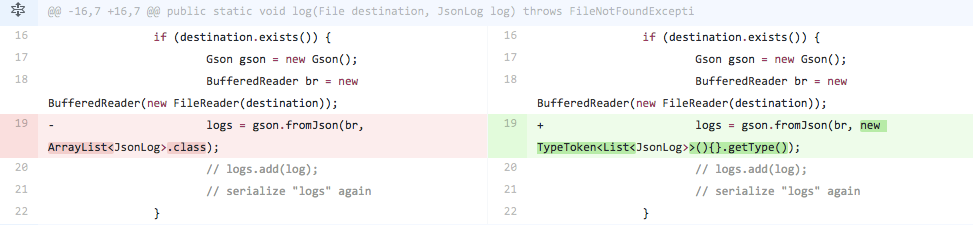
\includegraphics[width=\linewidth]{pull-request-1}
  \caption{Diff view for study scenario 1}
  \label{fig:pull-request-1}
\end{figure}

In (2), a developer was interested in how to compare version strings semantically. This question is associated with \textit{semantic versioning}\footnote{http://semver.org/} which defines what versions should be considered higher than others, i.e. \textit{1.0.0-alpha < 1.0.0-alpha.1 < 1.0.0-beta < 1.0.0-rc.1 < 1.0.0}. More specifically, the question was: \textit{given two version strings a and b, which one is higher?} For this scenario, we chose a lower ranked solution\footnote{http://stackoverflow.com/a/27891752/1105907} as a base version to be replaced by a higher ranked solution\footnote{http://stackoverflow.com/a/6640972/1105907} as the improved version. Both solutions are answers on the same given question on StackOverflow but in this case neither of the two is the accepted answer because the accepted answer in that case does not contain any code. Figures~\ref{fig:pull-request-2-1} and~\ref{fig:pull-request-2-2} show the diff of the change that we created for this scenario.

% TODO: say something why simple question-answer in scenario 1 but somewhat hidden answer content in scenario 2?

\begin{figure}[h]
  \label{fig:pull-request-2-1}
  \centering
  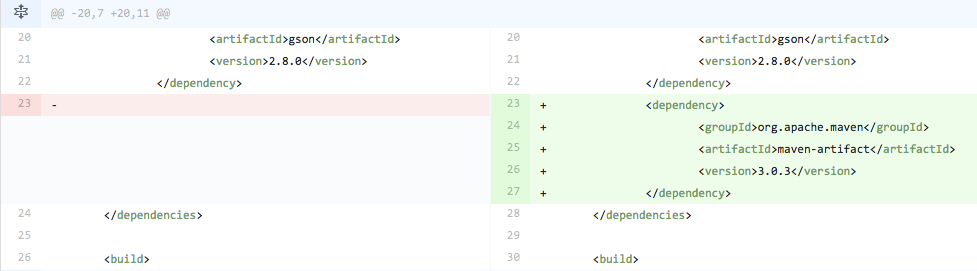
\includegraphics[width=\linewidth]{pull-request-2-1}
  \caption{Diff view for study scenario 2 (part 1)}
\end{figure}

\begin{figure}[h]
  \label{fig:pull-request-2-2}
  \centering
  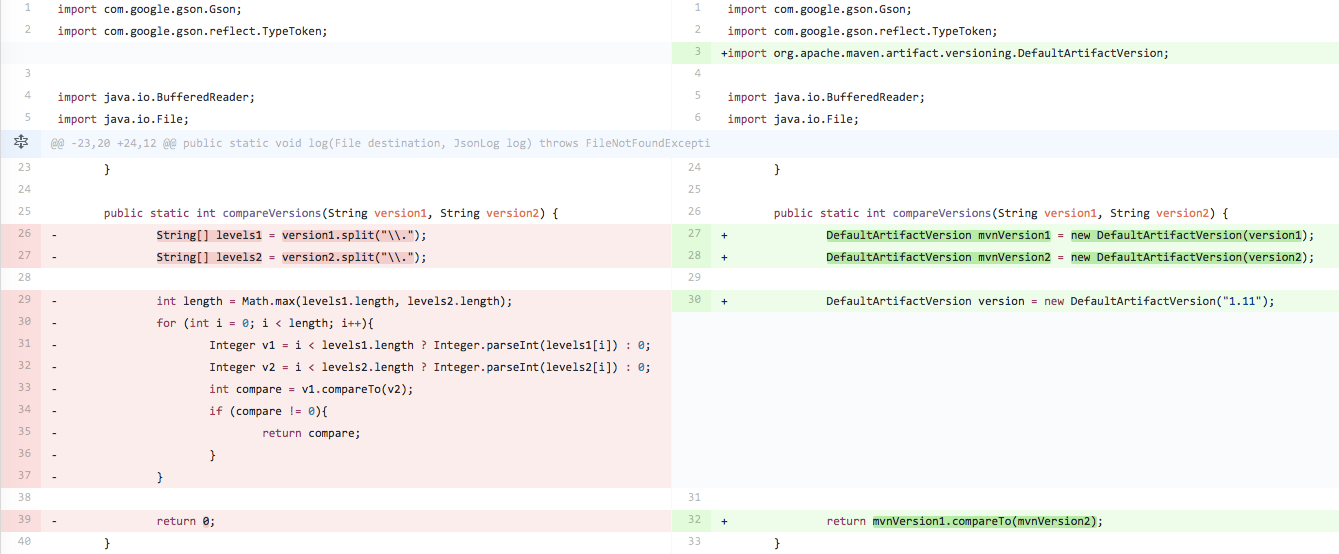
\includegraphics[width=\linewidth]{pull-request-2-2}
  \caption{Diff view for study scenario 2 (part 2)}
\end{figure}

For both scenarios we now added CodeStory to the developer workflow. The resulting CodeStory pages are shown in Figures~\ref{fig:codestory-page-1} and~\ref{fig:codestory-page-2}.

\begin{figure}[h]
  \label{fig:codestory-page-1}
  \centering
  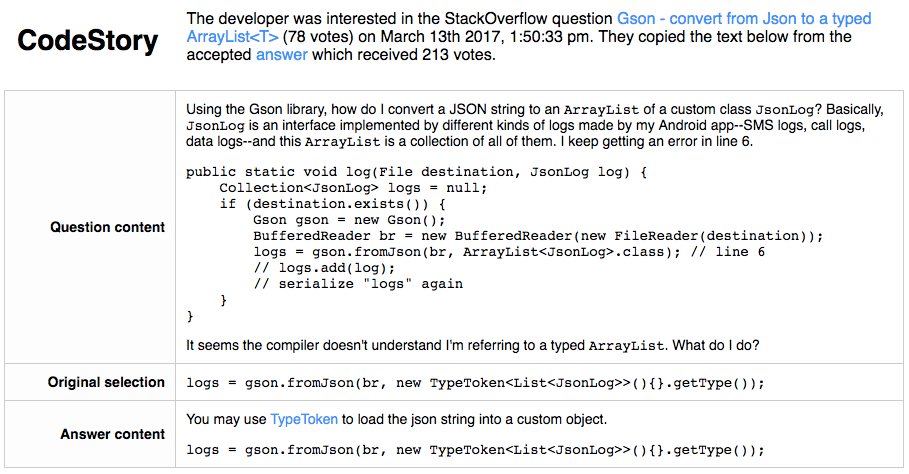
\includegraphics[width=\linewidth]{codestory-page-1}
  \caption{CodeStory page for scenario 1}
\end{figure}

\begin{figure}[h]
  \label{fig:codestory-page-2}
  \centering
  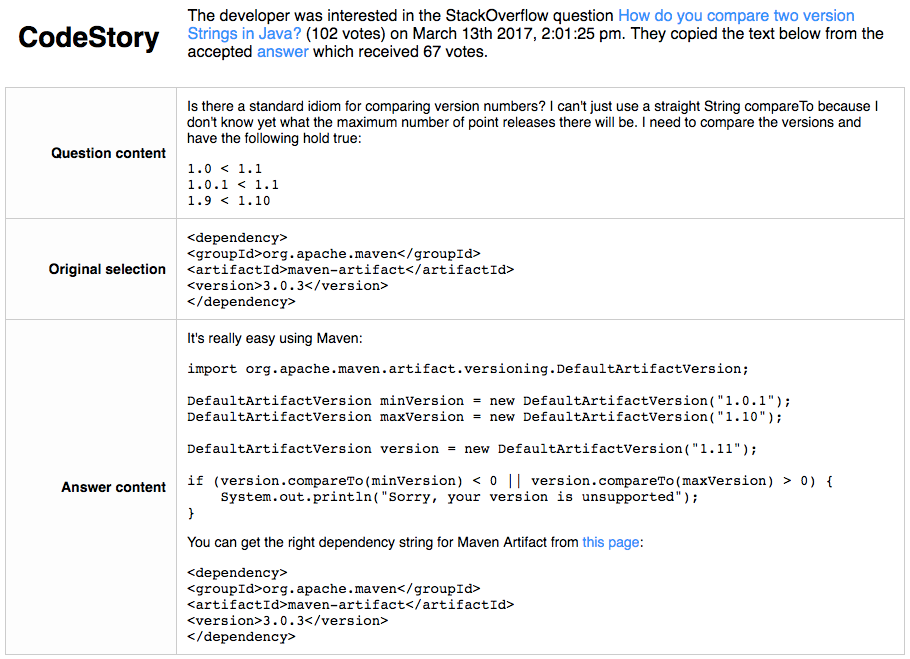
\includegraphics[width=\linewidth]{codestory-page-2}
  \caption{CodeStory page for scenario 2}
\end{figure}

For the changes described with scenario 1 and 2 we now created another version for each that includes a link to the respective CodeStory page as URL in a comment above the pasted content. Since scenario 2 contained two paste operations (one in an XML file and one in a Java file), two such comments were added respectively. This constellation gave us four treatments for our study:
\begin{itemize}
  \item \textbf{T1:} Scenario 1 without annotation
  \item \textbf{T2:} Scenario 2 without annotation
  \item \textbf{T3:} Scenario 1 with annotation
  \item \textbf{T4:} Scenario 2 with annotation
\end{itemize}

The study was performed with 8 developers among which 4 participants were graduate students and 4 were industry developers (> 4 years of practical experience with Java). With participants from different backgrounds we ensured generalizability of our study for both academia and industry. Due to time constraints we decided to assign each participant 2 code reviews (we assumed ~10min for each code review). To avoid learning bias for the given scenarios and treatments, we decided to let each participant do one code review for each scenario, one with annotation and one without annotation. To further avoid learning bias, we ensured that 4 participants start with a code review with annotation and the other 4 start with a code review without annotation. Table~\ref{tab:study-outline} shows the outline of treatments and participants.

\begin{table*}[t]
    \label{tab:study-outline}
    \centering
    \begin{threeparttable}
    \begin{tabular*}{\textwidth}{lll}
    \hline
    \textbf{Participant} & \textbf{Treatment} & \textbf{Background} \\
    \hline
    P1 & T3 + T2 & industry \\
    P2 & T3 + T2 & academia \\
    P3 & T1 + T4 & industry \\
    P4 & T1 + T4 & academia \\
    P5 & T4 + T1 & industry \\
    P6 & T4 + T1 & academia \\
    P7 & T2 + T3 & industry \\
    P8 & T2 + T3 & academia \\
    \hline
    \end{tabular*}
    \end{threeparttable}
    \caption{Study Outline}
\end{table*}

For each participant we forked our bootstrap repository and created two pull requests with respect to their treatments. In the description of each pull requests we asked the following questions:
\begin{enumerate}
  \item What is the purpose of the method with the change?
  \item How did the method change?
  \item Why was this change made?
\end{enumerate}

We then added the participants as reviewers and instructed them to perform their code reviews in sequential order by answering our questions as comments on the pull requests. The code reviews were thus performed online and no time constraints besides the sequential order were given since we did not see any benefits in imposing further restrictions on participants.

After the second pull request, participants were finally approached with a survey to determine to what degree CodeStory helped them during the code review (for the annotated pull request) and whether they found it useful. We first asked participants to rank their experience for each pull request on a scale from 1 (very challenging) to 5 (very easy). 

% TODO: tables!

For the first pull request (the JSON serialization scenario), 4 participants rated with 4 and 4 participants rated with 5 and there is no tendency regarding participants' backgrounds (i.e. students and industry developers rated the same). For the second pull request (the string version comparison scenario) there is more variance: 1 participant rated with 1, 4 participants rated with 2, 2 participants rated with 3 and 1 participant rated with 5.


\subsection{Impact for Code Review Tasks} \label{eval-impact}

\subsection{Threads to Validity} \label{eval-threats}

\end{document}
